\section{本章の概要}
コンセプトマップ\cite{concept}とは,ある領域における概念をノードとして,関連性のあるノード同士を線,すなわちリンクで繋げたグラフ表現の内の一つである.
リンクには,ノードとノード間の関係性を表すリンクキーワードが設定されることもある.
コンセプトマップを用いることで,概念間の関係は視覚的に整理される.
視覚的に整理されるため,階層構造の理解に有効であるとされている.

\section{コンセプトマップについて}
コンセプトマップは,様々な分野で利用されているが,主に理科教育においてよく用いられている\cite{yama}\cite{saito}.

\begin{figure}[htbp]
\begin{center}
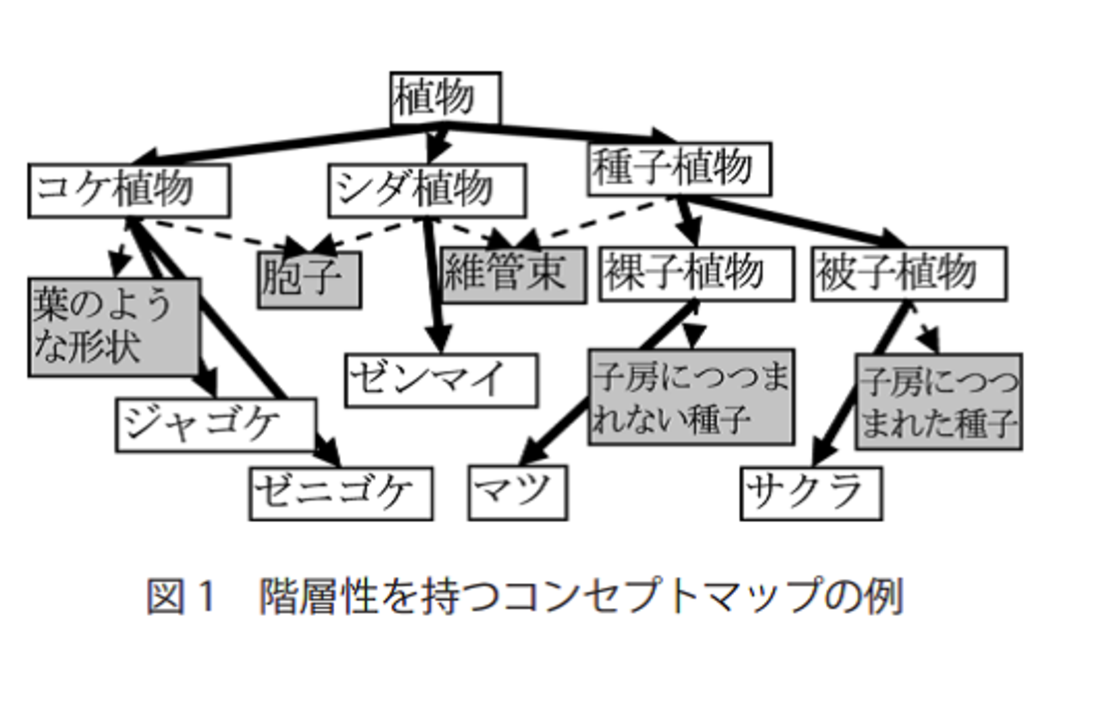
\includegraphics[width=8cm]{img/example_concept.eps}
\end{center}
\caption{コンセプトマップの例(出典: 誤りの可視化による階層構造の理解を指向したコンセプトマップ構築学習の支援環境 p.43 \cite{toumoto})}
\label{fig:example_concept}
\end{figure}

図\ref{fig:example_concept}は最上位の親を植物として,子にはコケ植物,シダ植物,種子植物が存在する,階層性のあるコンセプトマップである.
例えば種子植物に注目すると,その子である裸子植物,被子植物の間や,被子植物とサクラの間にも同様の親子関係が存在している.
また,コケ植物に注目すると,コケ植物には葉のような形状という独自の特徴すなわち属性を持っており,子であるジャゴケとゼニゴケにもその特徴は継承されている.
このようにして,コンセプトマップは概念間の関係性が可視化され,階層構造の理解に有効である.

一方コンセプトマップを学習の場で用いる場合大きく分け4つの形式が考えられる.
一つ目は,コンセプトマップを構築するテーマだけを与えられ,ノードとリンクを学習者が構築する形式.
二つ目は,コンセプトマップを構築するテーマと指導者側が学習者側に考慮してほしい概念をあらかじめ与えて,その他のノードやリンクを学習者に構築させる形式.
三つ目は,テーマとノードがすべて与えられて学習者はリンクのみを構築する形式.
四つ目は,テーマとあらかじめすべてのノードと一部のリンクが与えられ,残りのリンクのみを学習者が構築する形式.
本研究では,三つ目の形式で学習者にコンセプトマップを作成させた.
